% -*- mode: LaTeX; compile-command: "pdflatex CS-history.tex" -*-

\documentclass[xcolor={usenames,dvipsnames,svgnames,table},12pt]{beamer}

\mode<presentation>
{
  \usetheme{default}                          % use a default (plain) theme

  \setbeamertemplate{navigation symbols}{}    % don't show navigation
                                              % buttons along the
                                              % bottom
  \setbeamerfont{normal text}{family=\sffamily}

%  \setbeamertemplate{footline}[frame number]

  \AtBeginSection[]
  {
    \begin{frame}<beamer>
      \frametitle{}
      \begin{center}
        {\Huge \insertsectionhead}

        % \vspace{0.25in}
        % \includegraphics[width=2in]{\secimage}
      \end{center}
    \end{frame}
  }
}

\newenvironment{xframe}[1][]
  {\begin{frame}[fragile,environment=xframe,#1]}
  {\end{frame}}

% uncomment me to get 4 slides per page for printing
% \usepackage{pgfpages}
% \pgfpagesuselayout{4 on 1}[uspaper, border shrink=5mm]

% \setbeameroption{show only notes}

\usepackage[english]{babel}
\usepackage[T1]{fontenc}
\usepackage{graphicx}
\graphicspath{{images/}}

\usepackage{ulem}
\usepackage{url}
\usepackage{fancyvrb}

\title{Computer Science History}
% \date{}
% \author{Dr.\ Brent Yorgey}

%%%%%%%%%%%%%%%%%%%%%%%%%%%%%%%%%%%%%%%%%%%%%%%%%%%%%%%%%%%%%%%%%%%

\begin{document}

% \maketitle

\begin{frame}
  \begin{center}
    When was the first mechanical computer made?
  \end{center}
\end{frame}

\begin{frame}{Antikythera Mechanism}
  \begin{center}
    \raisebox{-0.5\height}{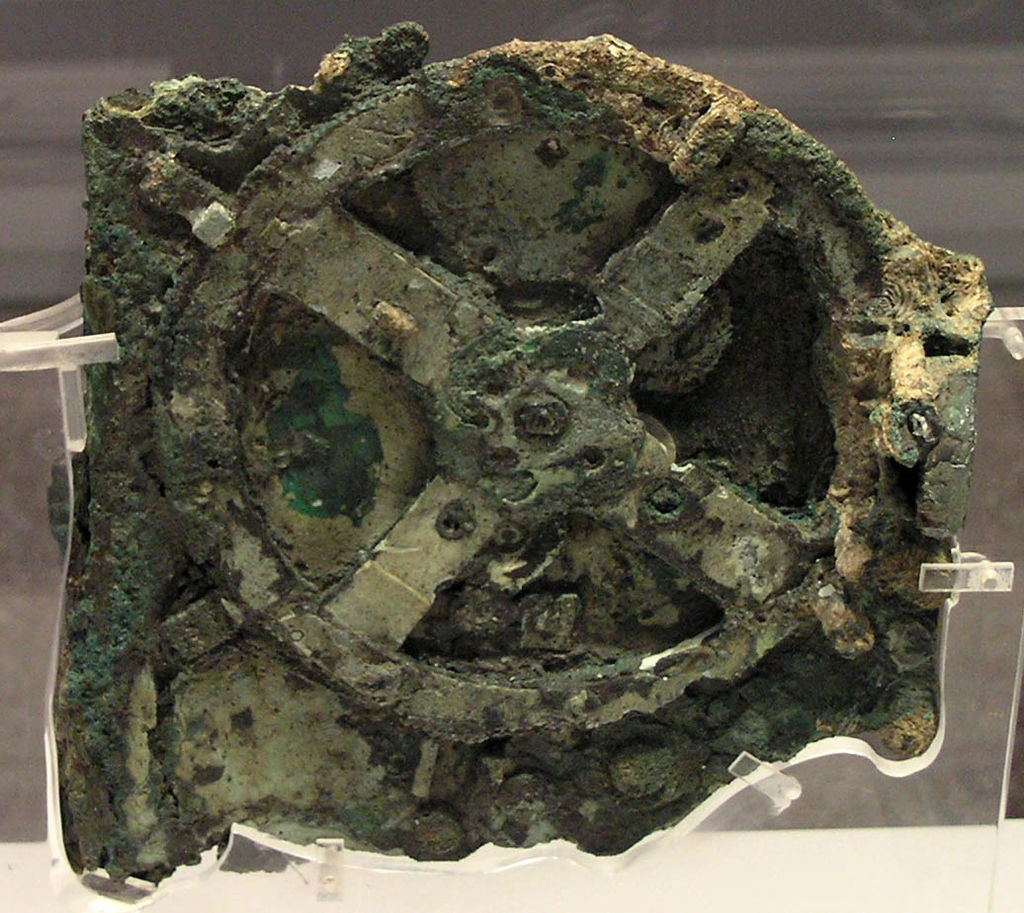
\includegraphics[width=2in]{antikythera1.jpeg}} \quad
    \raisebox{-0.5\height}{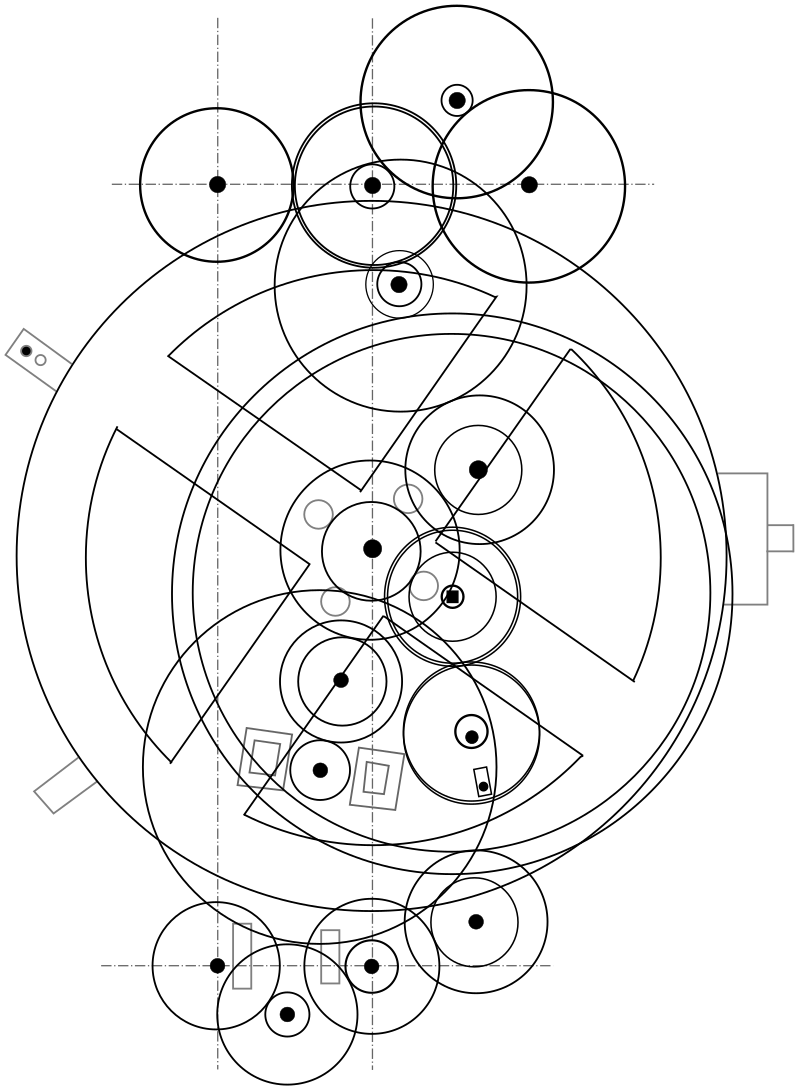
\includegraphics[width=2in]{Antikythera-gears.png}} \\
    100-200 BC?
  \end{center}
\end{frame}

\end{document}
